\scanpage{8}
Supposons que $q\alpha-\alpha'\ne0$ alors
\[
\begin{aligned}
(1)\ \Longrightarrow\quad &p\mid\sum_{i=1}^{q-1}C_q^i\,a^i b'^{\,q-i-1}+b'^{\,q-1}\\
\Longrightarrow\quad &p\mid q\,a^{q-1}\qquad\text{Car }p\mid b'\ \text{et pour }i\ne q-1\quad q-i-1\deleted{\ne0}>0
\end{aligned}
\]
or $p\mid b'$ et $b'\mid b^q$ donc $b'\mathrel{\underset{1}{\smile}}a$ donc $p\mathrel{\underset{1}{\smile}}a$

\deleted{donc si $\unsure{p\ne1|p\ne q}$}
\[
(1)\ \Longrightarrow\quad p\mid q\qquad\text{donc }\deleted{p=1\ \text{ou }}p=q\quad(\text{si }q\alpha-\alpha'\ne0)
\]
Donc si $p\ne q$ \quad
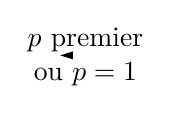
\begin{tikzpicture}[baseline=(p.base)]
\node[inner sep=0pt] (p) at (0,0) {$p$ premier};
\node[inner sep=0pt,anchor=north] at (0,-.28) {\inserted{ou $p=1$}};
% Small dark triangular mark above the addition; its guiding function is uncertain.
\fill (-.32,-.20) -- (-.16,-.15) -- (-.16,-.25) -- cycle;
\end{tikzpicture}
et $p\mid b'$ alors $\alpha'=q\alpha$
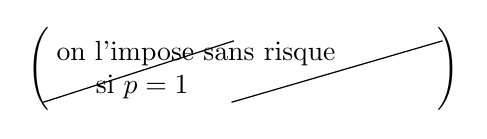
\begin{tikzpicture}[baseline=(u.base)]
\node[inner sep=0pt,anchor=west] (u) at (.22,0)
 {\rlap{on l'impose sans risque}\phantom{\deleted{on l'impose sans risque}}};
\node[inner sep=0pt,anchor=west] (v) at (.72,-.42)
 {\rlap{si $p=1$}\phantom{\deleted{si $p=1$}}};
\node[inner sep=0pt] at (0,-.20)
 {\rlap{$\Bigg($}\phantom{\deleted{$\Bigg($}}};
\node[inner sep=0pt] at (5.2,-.20)
 {\rlap{$\Bigg)$}\phantom{\deleted{$\Bigg)$}}};
% Two separate oblique cancellations over the two-line parenthesis.
\draw[line width=.45pt] (.06,-.62) -- (2.48,.16);
\draw[line width=.45pt] (2.45,-.62) -- (5.13,.16);
\end{tikzpicture}

Donc $\exists\,b_0\in\mathbb N^*$ et $\exists\,\gamma\in\mathbb N$ tel que $b'=q^\gamma b_0^q$ \margin{$q\nmid b_0$}

de plus $b_0\mid b$ et si $b=b_0 b''$ alors $b_0\mathrel{\underset{1}{\smile}}b''$ ?

De même $\exists\,a_0\in\mathbb N^*$ et $\exists\,\unsure{\zeta|\delta}\in\mathbb N$ tel que $a'=q^\zeta a_0^q$ avec $a_0\mid a$ et si $a=a_0a''$ alors $a_0\mathrel{\underset{1}{\smile}}a''$ ?

or $a\mathrel{\underset{1}{\smile}}b\Longrightarrow a_{\deleted{\unsure{0}}}'\mathrel{\underset{1}{\smile}}b'\Longrightarrow\zeta\times\gamma=0$ (et aussi $a_0\mathrel{\underset{1}{\smile}}b_0$)

Je suppose désormais que $\zeta=0$ donc $a'=a_0^q$

\figure{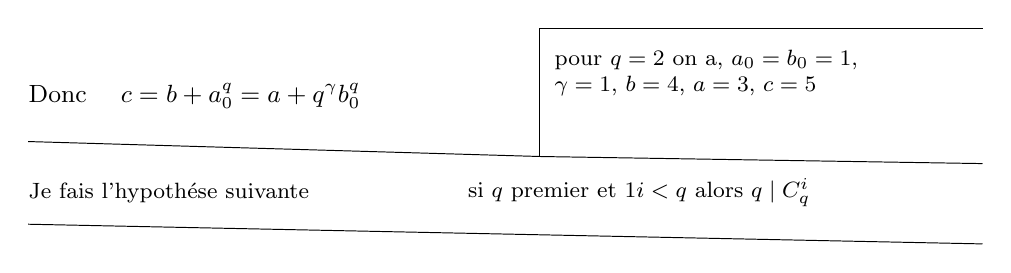
\begin{tikzpicture}[x=1cm,y=1cm]
\node[anchor=west,inner sep=0pt,font=\small] at (0,.80)
 {Donc \quad $c=b+a_0^q=a+q^\gamma b_0^q$};
\node[anchor=north west,inner sep=0pt,font=\footnotesize] at (6.68,1.43)
 {\begin{tabular}{@{}l@{}}
 pour $q=2$ on a, $a_0=b_0=1$,\\
 $\gamma=1$, $b=4$, $a=3$, $c=5$
 \end{tabular}};
% Open right border; the left edge meets the shared long upper rule.
\draw[line width=.35pt] (12.12,1.66) -- (6.50,1.66) -- (6.50,.03);
\draw[line width=.35pt] (0,.22) -- (6.50,.03) -- (12.12,-.06);
\node[anchor=west,inner sep=0pt,font=\footnotesize] at (0,-.43)
 {Je fais l'hypothése suivante};
\node[anchor=west,inner sep=0pt,font=\footnotesize] at (5.58,-.43)
 {si $q$ premier et $1\leqslant i<q$ alors $q\mid C_q^i$};
\draw[line width=.35pt] (0,-.83) -- (12.12,-1.08);
\end{tikzpicture}}
alors Si $q\geqslant3$ et $q\alpha-\alpha'\geqslant2$ \deleted{\unsure{alors}} on a \inserted{$p=q,\ {\unsure{a|\alpha}}'=\gamma$}
\[
\begin{aligned}
(1)\ \Longrightarrow\quad
 &\deleted{\unsure{p^{2}|p}}q^2\mid q\,a^{q-1}\quad
 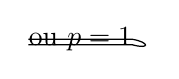
\begin{tikzpicture}[baseline=(d.base)]
 \node[inner sep=0pt] (d) at (0,0)
  {\rlap{ou $p=1$}\phantom{\deleted{ou $p=1$}}};
 \draw[line width=.45pt] (d.west) -- (d.east)
  .. controls +(0.22,-.04) and +(0.22,-.06) ..
  ([yshift=-2pt]d.east) -- ([yshift=-2pt]d.west);
 \end{tikzpicture}\\[.8ex]
\Longrightarrow\quad
 &q\mid a^{q-1}\quad
 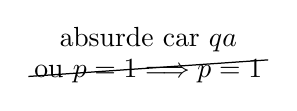
\begin{tikzpicture}[baseline=(d.base)]
 \node[inner sep=0pt] (d) at (0,0)
  {\rlap{ou $p=1\Longrightarrow p=1$}\phantom{\deleted{ou $p=1\Longrightarrow p=1$}}};
 \draw[line width=.45pt] ([xshift=-2pt,yshift=-2pt]d.west)
  -- ([xshift=2pt,yshift=4pt]d.east);
 \node[inner sep=0pt,anchor=south] at (0,.23)
  {\inserted{absurde car $q\nmid a$}};
 \end{tikzpicture}
\end{aligned}
\]
Donc $\gamma=0$ ou $\gamma=$
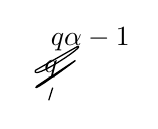
\begin{tikzpicture}[baseline=(q.base)]
\node[inner sep=0pt] (q) at (0,0)
 {$\rlap{$q$}\phantom{\deleted{q}}$};
% The live entry is physically raised above and to the right of the cancelled q.
\node[inner sep=0pt,anchor=south west] at (-.01,.22) {$q\alpha-1$};
\draw[line width=.45pt] (-.20,-.02) -- (.33,.28)
 .. controls (.48,.32) and (-.26,-.17) .. (-.20,-.02);
\draw[line width=.45pt] (-.18,-.22) -- (.30,.10)
 .. controls (.39,.16) and (-.29,-.34) .. (-.18,-.22);
\draw[line width=.45pt] (.02,-.24) -- (-.03,-.40);
\end{tikzpicture}
(sous réserve que l'hypothése est vraie)%
\margin{\begin{tikzpicture}[baseline=(n.base)]
\node[inner sep=0pt,text width=.85\marginparwidth] (n)
 {C'est peut-être interessant car ici $2$ est mis à part dans
 \(\mathord{\overset{\scriptscriptstyle\unsure{/}}{\vphantom{l}}}\)l'ensemble des nombres premiers};
% Small detached rising stroke before l'ensemble: role and hand unresolved.
% Return arrow rises at the right from the final parenthesis toward this note.
\draw[->] ([yshift=-.25cm]n.south east) -- ++(.16,0) |- (n.north east);
\end{tikzpicture}}
% archive sheet number: 7
